\documentclass[../main/main.tex]{subfiles}

\newdate{date}{09}{12}{2020}

% \begin{figure}[h!]
% \centering
% \includegraphics[page=6,width=0.8\textwidth]{../lessons/pdf_file/23_lecture.pdf}
% \end{figure}

%\displaydate{date}. Compiled:  \today. Alice.

\begin{document}

\pagestyle{plain}

\section{Lecture 23}


\subsubsection*{Slide 1}

\begin{minipage}[]{0.5\linewidth}
\centering
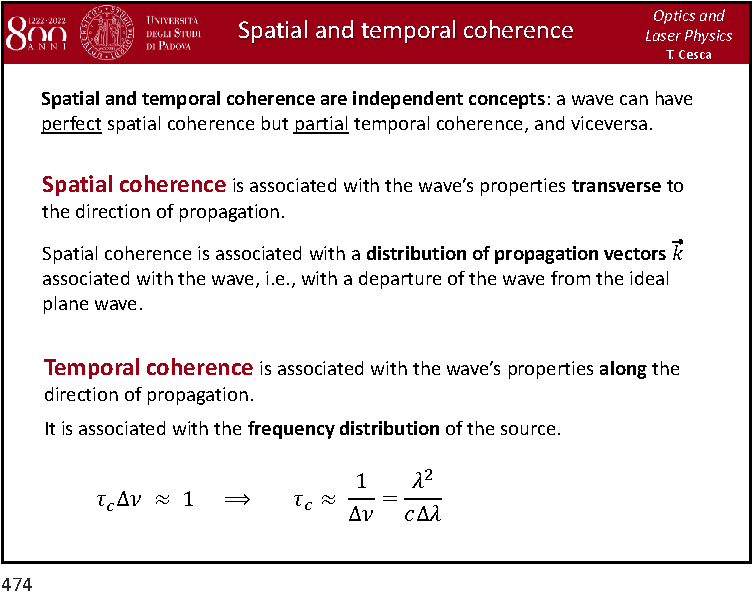
\includegraphics[page=1,width=1\textwidth]{../lessons/pdf_file/23_lecture.pdf}
\end{minipage}
\hspace{0.3cm}\vspace{0.3cm}
\begin{minipage}[c]{0.47\linewidth}

Temporal coherence is more related to monocromaticity.

\end{minipage}

\subsubsection*{Slide 2}

\begin{minipage}[]{0.5\linewidth}
\centering
\includegraphics[page=2,width=1\textwidth]{../lessons/pdf_file/23_lecture.pdf}
\end{minipage}
\hspace{0.3cm}\vspace{0.3cm}
\begin{minipage}[c]{0.47\linewidth}

The \textbf{first-order auto-correlation function} gives information on temporal coherence.

\( T \) is the period of oscillation of our wave.

The real part of \( g^{(1)} \) is an oscillating function! The amplitude of this function will be modulated by the term in the brackets.

\end{minipage}

\subsubsection*{Slide 3}

\begin{minipage}[]{0.5\linewidth}
\centering
\includegraphics[page=3,width=1\textwidth]{../lessons/pdf_file/23_lecture.pdf}
\end{minipage}
\hspace{0.3cm}\vspace{0.3cm}
\begin{minipage}[c]{0.47\linewidth}

\( \tau _c \) is the correlation time.


\end{minipage}

\newpage

\subsubsection*{Slide 4}

\begin{minipage}[]{0.5\linewidth}
\centering
\includegraphics[page=4,width=1\textwidth]{../lessons/pdf_file/23_lecture.pdf}
\end{minipage}
\hspace{0.3cm}\vspace{0.3cm}
\begin{minipage}[c]{0.47\linewidth}

If \( \tau  \) is increasing the relation between the phases become random.

\end{minipage}

\subsubsection*{Slide 5}

\begin{minipage}[]{0.5\linewidth}
\centering
\includegraphics[page=5,width=1\textwidth]{../lessons/pdf_file/23_lecture.pdf}
\end{minipage}
\hspace{0.3cm}\vspace{0.3cm}
\begin{minipage}[c]{0.47\linewidth}

The shape of \( g^{(1)} \) depends on the spectral broadening.

If we have homogeneous broadening, we have that the first-order correlation function can be calculated in this way.

\end{minipage}

\subsubsection*{Slide 6}

\begin{minipage}[]{0.5\linewidth}
\centering
\includegraphics[page=6,width=1\textwidth]{../lessons/pdf_file/23_lecture.pdf}
\end{minipage}
\hspace{0.3cm}\vspace{0.3cm}
\begin{minipage}[c]{0.47\linewidth}

If we have inhomogeneous broadening, we have a function like this.

\end{minipage}

\newpage

\subsubsection*{Slide 7}

\begin{minipage}[]{0.5\linewidth}
\centering
\includegraphics[page=7,width=1\textwidth]{../lessons/pdf_file/23_lecture.pdf}
\end{minipage}
\hspace{0.3cm}\vspace{0.3cm}
\begin{minipage}[c]{0.47\linewidth}

The problem is how to obtain \( \tau _c \) from an experimental point of view. To determine the auto-correlation function we can use a Michelson interferometer.

\end{minipage}

\subsubsection*{Slide 8}

\begin{minipage}[]{0.5\linewidth}
\centering
\includegraphics[page=8,width=1\textwidth]{../lessons/pdf_file/23_lecture.pdf}
\end{minipage}
\hspace{0.3cm}\vspace{0.3cm}
\begin{minipage}[c]{0.47\linewidth}

It can be schematized in this way. We send the input beam on a beam splitter which divide the amplitude of the beam in 50$\%$. We have one mirror in each arm.

We can vary the distance of the second mirror.

The output will produce fringe of interference. If we move the second mirror, the fringes are moving. By analyzing the evolution of the fringes as a function of \( L_2 \) we can characterize the beam.

\( \Delta \Phi  \) is an extra phase which take into account the phase-shift introduced by the path or any other possibility (for instance reflection at the beam splitter or the presence of coatings and so on...).

\end{minipage}

\subsubsection*{Slide 9}

\begin{minipage}[]{0.5\linewidth}
\centering
\includegraphics[page=9,width=1\textwidth]{../lessons/pdf_file/23_lecture.pdf}
\end{minipage}
\hspace{0.3cm}\vspace{0.3cm}
\begin{minipage}[c]{0.47\linewidth}

The intensity can be described by this cosin function of \( \delta  \). We apply the condition to get maxima of interference and minima.

We can introduce also the \textbf{fringe visibility}.

\end{minipage}

\subsubsection*{Slide 10}

\begin{minipage}[]{0.5\linewidth}
\centering
\includegraphics[page=10,width=1\textwidth]{../lessons/pdf_file/23_lecture.pdf}
\end{minipage}
\hspace{0.3cm}\vspace{0.3cm}
\begin{minipage}[c]{0.47\linewidth}

Let us see how we can link the Michelson interferometer to compute the auto-correlation function.

The intensity that we can measure as a function of \( \tau  \) is related to the first-order auto-correlation function.

\end{minipage}

\subsubsection*{Slide 11}

\begin{minipage}[]{0.5\linewidth}
\centering
\includegraphics[page=11,width=1\textwidth]{../lessons/pdf_file/23_lecture.pdf}
\end{minipage}
\hspace{0.3cm}\vspace{0.3cm}
\begin{minipage}[c]{0.47\linewidth}

We can relate the fringe visibility with the first-order auto-correlation function.

By changing \( L_2 \), we change \( \tau  \) so we can compute \( \abs{g_1 (\tau )}  \).

\end{minipage}

\subsubsection*{Slide 12}

\begin{minipage}[]{0.5\linewidth}
\centering
\includegraphics[page=12,width=1\textwidth]{../lessons/pdf_file/23_lecture.pdf}
\end{minipage}
\hspace{0.3cm}\vspace{0.3cm}
\begin{minipage}[c]{0.47\linewidth}

If the aomplitudes of the electric field are different we have this more complex formula.

\end{minipage}

\subsubsection*{Slide 13}

\begin{minipage}[]{0.5\linewidth}
\centering
\includegraphics[page=13,width=1\textwidth]{../lessons/pdf_file/23_lecture.pdf}
\end{minipage}
\hspace{0.3cm}\vspace{0.3cm}
\begin{minipage}[c]{0.47\linewidth}

In this way we can distinguish the property of our light beam.

The most real case is \textbf{chaotic light} or \textbf{incoherent light}.

\end{minipage}

\subsubsection*{Slide 14}

\begin{minipage}[]{0.5\linewidth}
\centering
\includegraphics[page=14,width=1\textwidth]{../lessons/pdf_file/23_lecture.pdf}
\end{minipage}
\hspace{0.3cm}\vspace{0.3cm}
\begin{minipage}[c]{0.47\linewidth}

Let us give some numbers.

Important point: \textbf{temporal coherence is related to the bandwidth!}

\end{minipage}

\subsubsection*{Slide 15}

\begin{minipage}[]{0.5\linewidth}
\centering
\includegraphics[page=15,width=1\textwidth]{../lessons/pdf_file/23_lecture.pdf}
\end{minipage}
\hspace{0.3cm}\vspace{0.3cm}
\begin{minipage}[c]{0.47\linewidth}

In the same way, we can define a \textbf{first-order cross-correlation function} for the spatial coherence. The only difference is that we have to evalute the electric field at the position \( x_1 \) and \( x_2 \).

This is the same way for a Young interference.
Interference between two waves that are passing in the positions \( x_1 \) and \( x_2 \).

\end{minipage}

\subsubsection*{Slide 16}

\begin{minipage}[]{0.5\linewidth}
\centering
\includegraphics[page=16,width=1\textwidth]{../lessons/pdf_file/23_lecture.pdf}
\end{minipage}
\hspace{0.3cm}\vspace{0.3cm}
\begin{minipage}[c]{0.47\linewidth}

We can have also in this case \textbf{full coherence}, \textbf{partial coherence} and \textbf{incoherence}.

You have to calculate \textbf{at the same time} the cross-correlation function!

While for the temporal coherence was \textbf{at the same position}!

\end{minipage}

\subsubsection*{Slide 17}

\begin{minipage}[]{0.5\linewidth}
\centering
\includegraphics[page=17,width=1\textwidth]{../lessons/pdf_file/23_lecture.pdf}
\end{minipage}
\hspace{0.3cm}\vspace{0.3cm}
\begin{minipage}[c]{0.47\linewidth}

Now, let us look at the \textbf{second-order correlation function}. We obtain the information about the degree of second-order temporal coherence: we are looking at the second power of the electric field. So, we have considering the correlation between the intensity of the beam. How do the intensity are correlated at different time?

Let us assume a \textbf{constant average intensity}. So, we can write the intensity at each time as the average value and fluctuations around the average value.

If \( \tau \gg \tau _c \) the fluctuations of the intensity are uncorrelated.

\end{minipage}

\subsubsection*{Slide 18}

\begin{minipage}[]{0.5\linewidth}
\centering
\includegraphics[page=18,width=1\textwidth]{../lessons/pdf_file/23_lecture.pdf}
\end{minipage}
\hspace{0.3cm}\vspace{0.3cm}
\begin{minipage}[c]{0.47\linewidth}

If we calculate \( g^{(2)} \) it is equal to one.

\end{minipage}

\subsubsection*{Slide 19}

\begin{minipage}[]{0.5\linewidth}
\centering
\includegraphics[page=19,width=1\textwidth]{../lessons/pdf_file/23_lecture.pdf}
\end{minipage}
\hspace{0.3cm}\vspace{0.3cm}
\begin{minipage}[c]{0.47\linewidth}

Now, let us consider the case in which \( \tau \ll \tau _c \). If \( \tau = 0 \), we see that \( g^{(2)} \ge 1 \).

We have that \( I(t)^2 \) is always positive so we have that the numberator is larger than the denominator!

\end{minipage}

\subsubsection*{Slide 20}

\begin{minipage}[]{0.5\linewidth}
\centering
\includegraphics[page=20,width=1\textwidth]{../lessons/pdf_file/23_lecture.pdf}
\end{minipage}
\hspace{0.3cm}\vspace{0.3cm}
\begin{minipage}[c]{0.47\linewidth}

We can summarize it here.

The trend of the chaotic depends on the lineshape (homogeneous or inhomogeneous broadening).

In general the second-order correlation function is related to the first-order correlation function. This is \textbf{true for any classical source of light!}

\end{minipage}

\subsubsection*{Slide 21}

\begin{minipage}[]{0.5\linewidth}
\centering
\includegraphics[page=21,width=1\textwidth]{../lessons/pdf_file/23_lecture.pdf}
\end{minipage}
\hspace{0.3cm}\vspace{0.3cm}
\begin{minipage}[c]{0.47\linewidth}

We can use the second-order correlation function to distinguish between \textbf{coherent light} and \textbf{nunched light}. This is valid for a \textbf{classical} source of light.

We can have \textbf{antibunched light}. This is possible only for a \textbf{quantum} nature of light!

These are the distribution of number of photons over time (each black dot is a photon). Coherent light correspond to a distribution of random photons.
Bunched light means that we have a bunched distribution of photons.
For antibunched we have a regular distribution of photons over time, with a given distance between each other.

So, for second-order correlation function we can distinguish between classical and quantum light beam!

\end{minipage}

\subsubsection*{Slide 22}

\begin{minipage}[]{0.5\linewidth}
\centering
\includegraphics[page=22,width=1\textwidth]{../lessons/pdf_file/23_lecture.pdf}
\end{minipage}
\hspace{0.3cm}\vspace{0.3cm}
\begin{minipage}[c]{0.47\linewidth}

We can compute the second-order correlation function in terms of photons. It represent the condition probability of detecting a second photon at time \( t = \tau  \), given that we detected one at \( t=0 \).

It is possible realizing the second-order correlation function with the HBT configuration.

We have a beam of photons impinging on a 50:50 beam splitter. We have two detectors. We can evaluate how log after the start the stop occurs.

Let us send to this setup an \textbf{antibunched beam} (long temporal intervals between two consective photons).

We have 50:50 probability that the beam goes to the first or to the second detector.

Let us suppose that it arrives in D1, the counter starts. If we wait a lot of time we have a second photon which can reach the detector D2. The timer is stopped.

\end{minipage}

So, \( g^{(2)} \) is 0 at \( \tau = 0 \) (we cannot have at the same time the photon reaching the second detector).
But, if we wait long time the probability to have a photon in the second detector is increasing and so you have the stop event.

\subsubsection*{Slide 23}

\begin{minipage}[]{0.5\linewidth}
\centering
\includegraphics[page=23,width=1\textwidth]{../lessons/pdf_file/23_lecture.pdf}
\end{minipage}
\hspace{0.3cm}\vspace{0.3cm}
\begin{minipage}[c]{0.47\linewidth}

If we measure the second-order correlation function (how many stop event occur after a given start event and you create a histogram for time delay \( \tau  \)) we have this trend here.

\end{minipage}

\subsubsection*{Slide 24}

\begin{minipage}[]{0.5\linewidth}
\centering
\includegraphics[page=24,width=1\textwidth]{../lessons/pdf_file/23_lecture.pdf}
\end{minipage}
\hspace{0.3cm}\vspace{0.3cm}
\begin{minipage}[c]{0.47\linewidth}

For bunched light, we have a large probability if we detect an event of start an event after a very short delay. If you wait time, the probability is decreasing: out of the bunch we get no more photons.

\end{minipage}

\subsubsection*{Slide 25}

\begin{minipage}[]{0.5\linewidth}
\centering
\includegraphics[page=25,width=1\textwidth]{../lessons/pdf_file/23_lecture.pdf}
\end{minipage}
\hspace{0.3cm}\vspace{0.3cm}
\begin{minipage}[c]{0.47\linewidth}

The excited a Na beam with a laser.

To obtain antibunching light we need the emission from a single atom (so obtaining a single photon). If we have a single atom which is emitting with a radiative lifetime \( \tau _R \), the probability of getting the emission of two photons with \( \tau \ll \tau _R \) is very low.

\end{minipage}

\subsubsection*{Slide 26}

\begin{minipage}[]{0.5\linewidth}
\centering
\includegraphics[page=26,width=1\textwidth]{../lessons/pdf_file/23_lecture.pdf}
\end{minipage}
\hspace{0.3cm}\vspace{0.3cm}
\begin{minipage}[c]{0.47\linewidth}

There is large interesting in realizing single photons sources. We need a parameter that we can control from the outside to trigger the emission of a single photon.

Single-photon sources can be used in quantum information. The idea can be to have single-photon sources which are able to emit at room temperature and that can be triggered.

\end{minipage}


\end{document}
